\part{Computing Limitation}

字典对“限制”有很多解释,其中有“界限”和“令人恼怒的或无法忍受的事物”等意思,通过分析可以了解到,计算机硬件、计算机软件和我们要使用计算机解决的问题都对计算机的问题求解有限制,计算机科学发展到现在都无法回避的问题就是——计算的限制。

就像路障会阻断交通一样,这些硬件、软件和问题带来的限制也阻止了计算机中某些类型的处理。

\chapter{硬件的限制}

硬件带给计算的限制来自于几个因素。其一,数字本身是无限的,而计算机能表示的数字却是有限的,这种限制会导致算术运算错误,生成不正确的结果。其二,硬件就是硬件,也就是说,它是由易坏的机械部件和电子部件构成的,硬件部件会磨损。其三,在把数据从一个内部设备传递给另一个内部设备,或者从一台计算机传递到另一台计算机时会发生问题,造成信息损失。计算机科学的发展过程中分析了这每一种问题并提出了一些最小化它们的影响的策略。

\section{算术运算的限制}

计算机的硬件对整数和实数的表示法都有限制。

\subsection{整数}

在Pep/7中,运行算术运算的寄存器是16位的,如果只表示正数,它能存储的最大值是65535,如果既要表示正数,又要表示负数,它能存储的最大值是32767。

Pep/7是一台虚拟计算机,在真实的计算机中,如果计算机的字长是32位,那么它能表示的整数范围是$-2147483648$到$2147483647$。

有些硬件系统支持长字算术,从而将计算机的字长扩展到64位,这样计算系统可以表示的整数范围扩展到了$-9~223~372~036~854~775~808$到$9~223~372~036~854~775~807$,即使是这样的长度也不足以进行所有运算。

Henry~Walker在《The~limits~of~Computing》中引述了在棋盘中的每一个格子中按如下规则放置稻谷的例子:

\begin{compactitem}
\item 棋盘的第一格放1粒稻谷;
\item 棋盘的第二格放2粒稻谷;
\item 棋盘的第三格放4粒稻谷;
\item 棋盘的第四格放8粒稻谷;
\item 每个后继方格中的稻谷数量是前一格的两倍,直到64个棋盘格放完为止。
\end{compactitem}

这样就会发现第一行有$255(1+2+4+8+16+32+64+128)$粒稻谷,第二行有$65280$粒稻谷,第三行有$963040$粒稻谷,而后续进行下来,只是第$64$个格子就有$263$粒稻谷,约为$8\times 1018$粒,相当于$110000$亿蒲式耳。

通过这个例子可以知道,整数可以增长得非常快,增长得非常大。如果计算机字长为64位,只表示正数,那么最多只能表示第64个棋盘格中的稻谷数。如果想把64个棋盘格中的稻谷数加起来,计算机就做不到了,这样将会发生溢出。

一台计算机的硬件决定了它能表示的数字(整数和实数)的限制,不过用软件方法可以克服这种限制。例如,可以用一系列较小的数表示很大的数,下图展示了如果通过在每个字中放一位数字表示整数。

\begin{figure}[htbp]
\centering
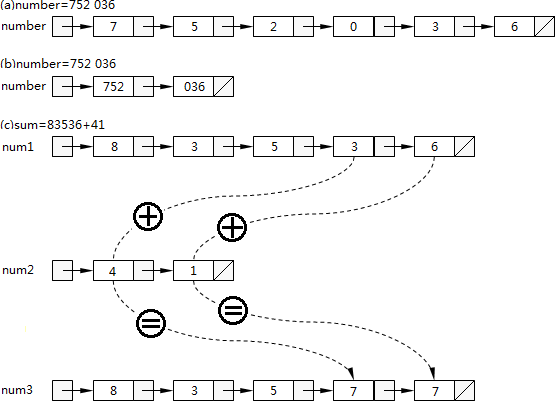
\includegraphics[height=220pt,keepaspectratio]{decimal.png}
\end{figure}

这样就可以实现用软件来表示非常大的数,操作这种形式的的整数的程序必须从最右边开始把每个数对相加,并且把进位加到左边一位的加法中。

\subsection{实数}

实数被存储为整数加说明小数点位置的信息。为了更好的理解为什么实数会带来问题,下面先看一个表示数字和小数点信息的编码模式。

为了便于讨论,我们假设计算机的内存单元大小相同,每个内存单元由一个符号和5个数字位组成。每当定义了一个变量或常量,赋予它的内存单元都由5个数字和一个符号构成。如果定义的是整数变量或整数常量,那么这个数会被直接存储起来。如果声明的是一个实数变量或实数常量,那么这个数将被存储为整数部分加小数部分,要表示这两部分,必须对该实数编码。

先了解编码后的数字是什么样的以及这些编码如何表示程序中的算术值,从整数开始。用5位数字能够表示的整数范围是-99999到+99999:

\begin{figure}[htbp]
\centering
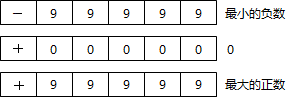
\includegraphics[height=60pt,keepaspectratio]{real.png}
\end{figure}

精度(precision,最多可以表示的有效位数)是5个数位。这个范围内的每个数都能被精确表示出来。如果用其中一个数位(如最左边的一位)表示指数则是下面的情况,例如:

\begin{figure}[htbp]
\centering
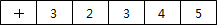
\includegraphics[height=15pt,keepaspectratio]{precision.png}
\end{figure}
表示的数字是$+2~345\times 10^3$,此时这5个数位表示的范围就大得多了,扩展到:
\[-9~999\times 10^9\mbox{到}+9~999×10^9\]
或
\[-9~999~000~000~000\mbox{到}+9~999~000~000~000\]
现在精度只有4位数字,也就是说,只能表示每个数中的4位有效位(signification digits,有效位指的是从左边的第一个非零数位开始,到右边的最后一个非零数位(或纯粹的零)结束的数字)。这意味着这个系统只能精确地表示4位数。对于更大的数会出现什么情况呢?

最左边的4位数字是正确的,其余的数字都被假设为0。右边的数位或者说最低有效数位将丢失。下面的例子说明了这种情况:

\begin{figure}[htbp]
\centering
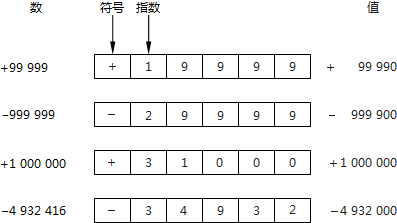
\includegraphics[height=120pt,keepaspectratio]{signification_digits.png}
\end{figure}

注意,我们只能精确地表示1000000,但不能精确地表示$-$4932416。我们的编码模式仅限于4位有效位,不能表示的数字被假设为0。

要扩展这种编码模式来表示实数,还要能够表示负指数,例如:
\[ 4394\times 10^{-2}=43.94\]
或
\[22×10^{-4}=0.0022\]
由于在我们的模式中,指数没有符号,所以必须对它稍加修改,把已经有的符号作为指数的符号,再在这个符号的左边加一个符号,作为数本身的符号。

\begin{figure}[htbp]
\centering
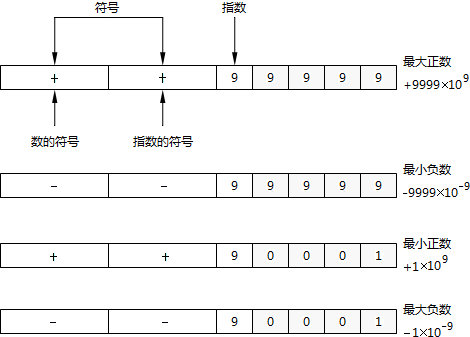
\includegraphics[height=200pt,keepaspectratio]{sign_number.png}
\end{figure}
现在可以表示$-9999×10^{-9}$到$9999×10^9$之间的所有数(精确到四位)了,包括所有的小数值。

假设想用这种编码模式求三个数$x$、$y$和$z$的和,可以先求$x$与$y$的和,再把$z$加到之前求得的结果上。也可以先求$y$与$z$的和,再把$x$加到之前求得的结果上。算术运算的结合律可以证明这两种方法得到的答案一样,但是真实的结果却未必。

计算机限制了实数的精度(有效位的位数)。下面用4位有效位加一位指数的编码模式求下列三个值的和:
\[ x=-1324\times 10^3~~y=1325\times 10^3~~z=5424\times 10^0\]
把$z$加到$x$和$y$的和上的结果如下:

\begin{table}[htbp]
\centering
\begin{tabular}{rrl}
$(x)$		& $-1324\times 10^3$ & 					\\
$(y)$		& $1325\times 10^3$	& 					\\
\hline
			& $1\times 10^3$		& $=1000\times 10^0$	\\
$(x+y)$	& $1000\times 10^0$	& 					\\
$(z)$		& $5424\times 10^0$	&					\\
\hline
			& $6424\times 10^0$	& $=(x+y)+z$	\\
\end{tabular}
\end{table}

把x加到y和z的和上的结果如下:

\begin{table}[htbp]
\centering
\begin{tabular}{rrl}
$(y)$		& $132500\times 10^0$	& 								\\
$(y)$		& $5424\times 10^0$		& 								\\
\hline
			& $1330424\times 10^0$	& $=1330\times 10^3$(截取4位有效数字)	\\
$(x+y)$	& $1330\times 10^3$	& 					\\
$(x)$		& $-1324\times 10^3$	&					\\
\hline
			& $6\times 10^3$	& $=6000\times 10^0=x+(y+z)$	\\
\end{tabular}
\end{table}

这两个答案的千位上的结果相同,但百位、十位和个位上的结果却不同,这叫做表示误差或舍入误差(representational(round-off)error),用来指代由于算术运算结果的精度大于机器的精度造成的算术误差。

$y$和$z$的和是精度为7位的数,但是只有4位被保存了下来。除了表示误差,浮点算术还有两个要注意的问题——下溢(underflow)和溢出(overflow)。当计算出的绝对值太小以至于给定的计算机不能表示时,将发生下溢。采用十进制数表示法,可以演示一个涉及到非常小的数的运算:

\begin{table}[htbp]
\centering
\begin{tabular}{rll}
$4210$			& $\times 10^{-8}$		& \\
$\times 2000$	& $\times 10^{-8}$		& \\
\hline
$8420000$		& $\times 10^{-16}$	& $=8420\times 10^{-13}$	\\
\end{tabular}
\end{table}

这个例子中的编码模式的最小指数是$-9$,而这时的指数$-13$太小了,所以不能表示这个数,因此这个运算的结果将被设为0。所有因为太小而不能表示的数都将被设为0。在这种情况下,这样做是合理的。

当计算出的绝对值太大以至于给定的计算机不能表示时,将发生溢出(overflow)。溢出是更加严重的问题。因为一旦发生溢出,没有合理的解决办法。例如,下列运算的结果:


\begin{table}[htbp]
\centering
\begin{tabular}{rll}
$9999$			& $\times 10^{9}$		& \\
$\times 1000$	& $\times 10^{9}$		& \\
\hline
$9999000$		& $\times 10^{18}$		& $=9999\times 10^{21}$	\\
\end{tabular}
\end{table}

在当前例子中的编码模式中就不能存储。而处理办法要与下溢的处理保持一致,可以把结果设置为$9999\times 10^9$,即模式中的最大实数值。而我们仅凭直觉也会发现这是不对的。另一种方法是停止运算报错。

浮点数可能发生的另一种错误是化零误差(cancellation error),由于计算机精度限制,当相加或相减的两个数的量级相差太大时会出现这种误差。下面是一个例子:
\[(1+0.00001234-1)= 0.00001234\]
算术运算的法则可以证明这个等式是正确的。但如果用计算机来执行这个运算却可能会出现下面的情况:

\begin{table}[htbp]
\centering
\begin{tabular}{rrl}
	& $100000000$	& $\times 10^{-8}$	\\
$+$& $1234$			& $\times 10^{-8}$	\\
\hline
	& $100001234$	& $\times 10^{-8}$	\\
\end{tabular}
\end{table}
因为只有4位精度,所以结果将变为$1000×10-3$。计算机再减去1:

\begin{table}[!h]
\centering
\begin{tabular}{rrl}
	& $1000$	&$\times 10^{-3}$	\\
$-$& $1000$	&$\times 10^{-3}$	\\
\hline
	& $0$			& 						\\
\end{tabular}
\end{table}

这是计算机的运算结果,是0而不是$0.00001234$。

在计算机的算术运算中,整数和实数,无论正数还是负数,都会发生溢出。另外要注意的是,第一,实数运算的结果通常与我们通常预期的不同。第二,如果处理的数非常大或非常小,要注意执行运算的顺序。

\section{部件的限制}

在计算机系统中,硬件故障的问题确实存在,硬盘可能会损坏,文件服务可能会崩溃,网络也可能会中断,于是J.A.N.Lee杜撰了Titanic效应这个词来形容系统崩溃的严重程度超出了设计者的想象力。硬件故障确实会发生,最后的解决方法是进行防御性维护。在计算领域,这意味着定期检测硬件的问题,替换损坏的零件。

防御性维护还要保证放置计算机的物理环境适宜,大型计算机常常需要具有空调和无尘的房间。PC也要求保持相应的运行环境。计算机科学中使用术语“bug”来表示计算机错误。后来,Edsger~Dijkstra反对使用这种术语,他认为这种叫法会使人们产生错觉以为计算机的错误超出了程序员的控制。他认为bug是一种智力欺骗,隐藏了程序自己制造错误的事实。

关于计算机部件限制的所有讨论都有一个前提,就是计算机硬件在设计和制造阶段都经过了全面的测试。

\chapter{通信的限制}

计算机之内和计算机之间的数据流是计算的生命血液。因此,一定要保证数据不被破坏。实现这一点的策略叫做检错码和误差校正码。检错码可以判断出在数据传输过程中是否发生了错误,并警告系统。误差校正码不仅能检测出发生的错误,还能判断出正确的值是什么。

\section{校验位}

校验位用于检测存储和读取或发送或接收一个字节的过程中发生的错误。校验位是在使用这种模式的硬件中的每个字节上加上了一个位。这个位用于确保9位数值(一个字节加一个校验位)中的1的个数是奇数(或偶数)。

奇数奇偶校验要求一个字节加一个校验位中有奇数个1。例如,如果一个字节中的值是11001100,那么校验位是1,这样才能得到奇数个1。如果字节中的值是11110001,那么校验位是0。

当从内存中读取或接收了一个字节时,将计算其中1的个数(包括校验位)。如果1的个数是偶数,说明发生了错误。如果硬件采用这种模式,每个字节将多一个附加位,只有硬件才能访问这个位,用于检测错误。偶数奇偶校验的模式与奇数奇偶校验的相同,只是其中必须有偶数个1。

\section{校验数位}

上述模式的一个软件变体是求一个字节中的每个数位的和,然后把和的个位与字节中的数存储在一起。例如,对于数字34376,每个数位的和是23,因此,存储的数就是34376$-$3。如果这个数中的4变成了3,就可以检测到错误。但是,如果7变成了6,而6变成了7,那么数位的和仍然是正确的,但是数却是错的。

这种模式可以扩展为多一个附加位,可以是奇数位的和的个位数。例如,34376可以存为34376$-$23,3是所有数位和的个位数,2是第1位、第3位和第5位的和的个位数。这种方法能捕捉到相邻数位之间的传输错误,但却会漏掉其他的传输错误。当然,还可以存储偶数位的和的个位数,也就是说,要检测的错误越重要,检测算法就越复杂。


\section{误差校正码}

如果对于一个字节或一个数保存了足够的信息,那么可以推导出错误的数位应该是什么。极端的冗余是对每个存储的值都保留两个独立的副本。如果发现奇偶校验或校验数位有错,那么可以查阅另一个副本以得到正确的值。当然,连个副本可能都有错。误差校正码主要用于硬盘驱动器或CD,CD表面的不完整性会破坏数据。

\chapter{软件的限制}

计算机软件(包括商业软件等)存在错误,这种问题并非由懒惰引起的,而是由软件的复杂度引起的。随着机器的功能越来越强大,计算机能够解决的问题也变得越来越复杂。以前一个问题由一个程序员解决,现在成了一个问题由一组程序员解决,最后一个问题由一组程序员组解决。

\section{软件的复杂度}

大型软件项目的大小和复杂度几乎一定会导致产生错误。虽然软件测试能够证明存在bug,但是不能证明不存在bug。我们可以测试软件,发现问题,修正问题,然后再测试软件。随着我们不断发现问题,解决问题,我们对软件的信心也会逐渐增强。但我们永远不能确保已经除去了所有的bug。软件中潜藏着其他的bug,我们还没有发现,这种可能性将一直存在。

Nancy~Leveson在《Communications~of~the~ACM》中指出过,20世纪60年代出现的计算分支软件工程的目标就是把工程原则引入软件开发。目前软件工程已经涉及到对抽象的角色的更深理解、模块性的引入以及软件生命周期的概念等。

虽然大多数概念来自工程学,但它们必须适合处理更抽象的数据时会发生的特殊问题。硬件设计受实现设计所用的材料的指导和限制,软件则主要受人类能力的限制,而不是物理限制。Leveson博士指出,“因此,前50年的特征是学习这个领域的限制,这与人类能够处理的复杂度的限制息息相关。”

构建软件的重点已经改变了。以前是构建新软件,而今天,现有软件的维护和升级的问题越来越多,逐渐占据了中央舞台。

随着计算机软件系统变得越来越大而且需要整组的程序设计人员,我们开始分析人类协作的方式,以便设计出能辅助人们有效协作的方法。

\subsection{当前提高软件质量的方法}

虽然不可能使大型软件系统完全没有错误,但是并不意味着我们应该放弃,我们可以采用某些策略来提高软件的质量。构建好的软件的最佳方法是从项目一开始就关注它的质量,应用软件工程的规则。


\subsection{软件工程}

以前在计算机问题求解的过程中,要经历三个阶段,即开发算法、实现算法和维护程序。而从定义明确的小任务转移到大型的软件项目,那么还需要增加两个阶段,即制定软件需求和规约。

软件需求(software~requirement)是用概括而精确的语句列出软件产品提供的功能。软件规约(software~specification)则详细说明了软件产品的功能、输入、处理、输出和特性,软件规约提供了设计和实现软件所必需的信息。软件规约说明了程序能够做什么,而不是怎么做。

Leveson博士把软件生命周期看作软件工程要规划的一部分。所谓软件生命周期指的不仅是编码,而是软件的开发和升级。因此,软件的生命周期包括下列阶段:
\begin{compactitem}
\item 需求分析;
\item 制定规约;
\item 设计(高层和低层);
\item 实现;
\item 维护。
\end{compactitem}

所有阶段都要执行验证操作。需求是否精确反映了需要的功能?规约是否精确反映了满足需求所需的功能?高层设计是否精确反映了规约中的功能?设计中的每个后继层是否精确实现了上一层的功能?代码实现是否与设计相符?维护阶段实现的改变是否精确反映了想要的改变?这些改变的实现是否正确?

在使用计算机解决实际问题时,随着问题的增大,验证操作也会变得越来越重要,越来越复杂。虽然设计和代码的测试是整个过程很重要的一部分,但也只是一小部分。在一个典型的项目中,有一半错误是在设计阶段发生的,而实现阶段发生的只是一半错误而已。这个数据会引起一些误解,如果以修正错误的代价为衡量标准,那么在设计过程中越早发现错误,修正错误的花费越小。

大型软件产品是由程序员组开发的,程序设计小组使用的两种有效验证方法是走查和审查。这些是正式的小组活动,目的是把揭露错误的责任从个人转移到小组。由于测试非常耗时,而且错误发现的越晚,代价越高,所以这种活动的目标是在测试开始前发现错误。

使用{\heiti 走查(walk-through)}的方法,将由一个小组用样本测试输入手动模拟设计或程序,在纸上或黑板上跟踪程序的数据。与全面的程序测试不同,走查并非要模拟所有可能的测试情况,它的目的只是模拟程序员选择的设计或实现程序需求的方法。

在{\heiti 审查(inspection)}过程中,将由一位读者(绝对不是程序的作者)逐行读出程序的需求、设计或代码。审查员会预先得到相关资料,而且预期会仔细阅读过这些资料。在审查过程中,审查员会根据审查报告中的记录指出错误之处。他们在预审时已经注释了许多错误。大声朗读的过程只是为了发现更多的错误。与走查一样,小组讨论的主要好处在于讨论是在所有小组成员之间进行的。程序员、测试员与其他小组成员的沟通会在测试开始前发现更多的程序错误。

因此,走查是由一个小组手动地模拟程序或设计的验证方法,而审查是由团队成员之一逐行读出设计,由其他成员负责指出错误的验证方法。

在高层设计阶段,要拿设计与程序需求进行比较,以确保设计方案包括了所有必需的功能,以及该程序或模块能够与系统中的其他软件正确地连接起来。在低层设计阶段,设计已经具有很多细节,在实现它之前,一定要进行预审。完成编码后,要再审查一次编译过的清单。审查(或走查)可以确保实现与需求和设计一致。成功地完成审查意味着可以开始程序测试了。

走查和审查都要以一种无威胁的方式执行。这些小组活动的重点是去除产品中的瑕疵,而不是设计或代码的作者采用的技术方法。由于这些活动的主持人都不是作者,所以针对的是错误,而不是人。

在过去的10年或15年中,Carnegie Mellon大学的软件工程学院在规范大型软件项目的审查过程的研究方面扮演了重要的角色。

SEI~Software~Engineering~Process~Group(SEPG)Conference上的1篇论文报告了一个项目,该项目采用小组走查和正式审查结合的方式能够把产品的错误减少86.6\%,这一过程要应用于生命周期的每个阶段。下表展示了在一个维护项目的生命周期的各个阶段发现的每1000行源代码(KSLOC)中的错误数。
\begin{table}[!h]
\centering
\caption{维护时发现的错误}
\begin{tabular}{|l|l|}
\hline
阶段					& KSLOC中的错误数				\\
\hline
系统设计				& 2								\\
\hline
软件需求				& 8								\\
\hline
设计					& 12								\\
\hline
代码审查				& 34								\\
\hline
测试活动				& 3								\\
\hline
\end{tabular}
\end{table}

在维护阶段,50多万行的程序被附加了40000行源代码。除了测试活动外,每个阶段都要进行正式的审查。

在软件工程中,对软件的规模进行了量化。Space~Shuttle~Ground~Processing~System具有50多万行代码;Windows 95具有1000万行代码。大多数大型项目的代码数介于这两者之间。

由于大型项目的复杂度,所以要编写没有错误的代码是不可能的。下面是预计错误量的一个参考标准:
\begin{compactitem}
\item 标准软件:每1000行代码25个bug;
\item 好的软件:每1000行代码2个错误;
\item Space~Shuttle软件:每10000行代码少于1个错误。
\end{compactitem}

E.N.Adams在《IBM~Journal~of~Research~and~Development》中估计到,在尝试删除大程序中的错误时,约有15\%$\sim$50\%的操作会引入新的错误。

在分析软件故障的过程中会发现,虽然可能的错误只有一种——编码错误,但是更深入追究下去,会发现严重的设计失误。几乎所有软件在特定条件下都会有意想不到的行为。这里的低级错误是由于缺乏软件工程的经验而构建了依靠软件进行安全操作的机器。此外,软件整体的不安全设计比某个编码错误重要得多。

\subsection{正式验证}

在计算机科学中,人们设想是否可以用工具来定位设计和代码中的错误,甚至可以不必运行程序就能进行验证。这种设想来自于几何学的比喻,我们不必对每个三角形都证明一次勾股定理,这说明该定理适用于我们用过的每个三角形。我们可以用数学方法证明几何定理,那么用类似的方法证明计算机程序同样可行。

程序正确性的验证独立于数据测试,是计算机科学理论研究的一个重要领域。这项研究的目标是建立证明程序的方法,就像证明几何定理的方法一样。现在已经有证明代码满足规约的必要方法,但是证明通常比程序本身更复杂。因此,验证研究的重点是尝试构建自动化的程序证明器,即验证其他程序的检验程序。

已经有正式的方法可以成功地验证计算机芯片的正确性。一个著名的例子是验证执行实数算术运算的芯片,这项验证获得了英国女王技术成就奖(Queen's~Award~for~Technological~Achievement)。牛津大学的程序设计研究组的组长C.A.R.Hoare与MOS~Ltd.一起对芯片是否满足规约进行了正式验证。同时执行的还有一种传统的测试方法。《Computing~Research~News》报道如下:
\begin{verbatim}
“正式的开发方法在两组之间的竞赛中取得了胜利,它只用了大约12个月的时间
就完成了,与预计的时间要短。此外,正式的设计指出了许多非正式设计经过几
个月的测试而没能指出的错误。最后的设计不仅质量更高,花费更小,完成得也
更快。”
\end{verbatim}
硬件层的正式验证技术的成功有望带来软件层验证的成功,但是,软件比硬件复杂得多,所以在不久的将来,不会出现太大的突破。

\subsection{开源运动}

在计算早期,软件(包括它的源代码)是与计算机绑定在一起的。从20世纪70年代开始,公司开始保留源代码,软件从而成为了一项大生意。

随着Internet的出现,世界各地的程序员可以轻易得到一个软件产品的简单的版本,而且程序员仍然对扩展或改进程序充满兴趣。跟踪项目进展的“善意独裁者”掌控者大部分开源项目。如果一种改变或改进获得了同辈开发人员的认可,加入了新的软件版本,那么它一定更出色。

Linux是最著名的开源项目,Linus~Torvolds以UNIX为蓝图,开发了这种操作系统的第一个简单版本,并且一直在观察着它的发展。Linux更像一个即将出现的模式的教科书示例。开源运动是一个大规模的奇迹,SourceForge是一个开发者的Web站点,现在已经具有18000多个开源项目,145000个程序员在为此忙碌着。


\section{臭名昭著的软件错误}

计算领域中的每个人都有自己喜欢的软件恐怖故事。这里只列出一些小例子。

1990年1月,AT\&T的长途电话网络由于电子交换系统的软件错误中断了9个小时。那天AT\&T收到了1.48亿个长途电话和800电话,只有50\%被转接了出去。这次故障还引起了数不清的间接破坏:
\begin{compactitem}
\item 宾馆丢失了预订电话。
\item 汽车出租代理丢失了租车电话。
\item 美国在线的预订系统通信量降低了2/3。
\item 电话推销商估计损失75000美元。
\item MasterCard不能处理200000个信贷批准。
\item AT\&T损失了6000万到7500万美元。
\end{compactitem}

正如AT\&T的主席Robert~Allen所说的,“这是我从商32年来最可怕的噩梦。”

怎么会出现这种情况呢?交换软件的早期版本是能够正确运行的。升级后的系统代码中的软件错误使它对故障交换响应得更快。这个错误发生在一个C代码的break语句中。像Henry~Walker在《The~Limits~of~Computing》中指出的,这次崩溃说明了许多软件故障的共同点。

在该软件发布之前,它已经经过大量的测试,而且已经正确运行了一个月。除了测试外,研发过程中还进行过代码检阅。一位程序员犯了这个错误,但是其他检阅代码的程序员却没注意到这个错误。一个相对罕见的事件序列触发了这次故障,这是事先很难预料得到的。而这个错误出现在为改进一个正确运行的系统而设计的代码中,即出现在维护阶段。

一位美国空军的监察员发现,美国核导弹舰队的关键部分和部件的计算机跟踪中出现了令人费解的错误。这些错误包括重复的、遗漏的和不正确的序列码,遗漏的和不正确的零件编号,以及不正确的设备数量和位置。10个发组井在要发射导弹时电量不足。监察员认为这些问题源自于系统缺乏输入和检测盘点数据的训练。这是GIGO(garbage~in, garbage~out,无用输入无用输出)的一个好例子。

另外,即使软件系统操作正确,如果使用的数据不好,答案也会错误。使用的数据好坏决定了答案的好坏。这种情况就是GIGO,即无用输入,无用输出。在心情一样地情况下,让人困惑的系统使用起来也更容易出错。

流传最广的软件事故与一台计算机化的放射治疗仪Therac-25有关,在1985年6月到1987年1月之间,Therac-25造成了6次重大的用药过量事故,导致了病人死亡或严重受伤。这些事故据说是应用医疗加速器35年以来最严重的放射事故。

深入分析软件故障时会发现,虽然可能的错误只有一种——编码错误,但是深入追究下去,会发现严重的设计失误。Leveson和Turner在《KIEEE~Computer》发表的文章中加入了下面的评论:
\begin{verbatim}
“从Therac-25的故事可以得到的教训是仅仅关注个别的软件bug不能保证系统安全。
几乎所有软件在特定条件下都会有意想不到的行为。这里的低级错误是由于缺乏
软件工程的经验而构建了依靠软件进行安全操作的机器。此外,软件整体的不安全
设计比某个编码错误重要得多。”
\end{verbatim}

1991年2月25日,海湾战争期间,一枚飞毛腿导弹击中了美国陆军的军营,有28名士兵死亡,100多人受伤。由于软件错误,位于沙特阿拉伯Dhahran的美国爱国者导弹发射器没能成功跟踪并阻截伊拉克的飞毛腿导弹。不过这个错误不是编码错误,而是设计错误。其中的一个运算涉及到1/10的乘法,这个数在二进制中是无尽的。在100个小时的发射操作中,这种算术错误累积的误差是0.34秒,足够使导弹偏离它的目标。

审计院总结道:
\begin{verbatim}
“爱国者从来没有阻击过飞毛腿导弹,而且我们也没有预计它要连续运行这么长时间。
事故发生两周前,陆军官方收到的以色列数据说明在系统连续运行了8小时后,已经
出现了误差。于是陆军官方修改了软件,以提高系统的精确性。但是直到2月26日,
飞毛腿导弹事件发生后的第二天,修改好的软件才到达Dhahran。”
\end{verbatim}

Gemini~V的着陆地点距预计的点100英里。什么原因?是导航系统的设计没有将地球围绕太阳的转动考虑在内。

1999年10月,美国发射的火星气候轨道探测器(Mars~Climate~Orbiter)进入了火星大气层,进入点比预计的低100公里,导致飞船烧掉了。火星气候轨道探测器任务失败调查小组的主席Arthur~Stephenson总结道:
\begin{verbatim}
“导致太空船销毁的根本原因是一个地面导航软件没能像NASA宣布的那样把英语
转换成度量单位……失败调查小组还发现了其他导致错误的重要因素,它们使错误
拖延下来,结果使飞船进入火星的路径出现了很大的误差。”
\end{verbatim}

1962年7月美国发射的水手1号(Mariner~1)金星探测器几乎一发射就转变了航向,不得不被销毁了。这个问题是由下面这行Fortran代码引起的:
\begin{verbatim}
DO 5 K=1.3
\end{verbatim}
其中的句号应该是个逗号。由于这个输入错误,价值1850万美元的太空探索飞船就这么毁掉了。

软件错误并不只是美国政府才会犯。

1996年6月4日,欧洲空间局发射的无人火箭Ariane5在升空40秒后就爆炸了。这架火箭开发了十几年,开发费是70亿美元。火箭本身和它携带的货物价值5亿美元。究竟发生了什么问题呢?一个相对于平台的水平速率是64位的浮点数大于32767,结果被转换成了16位的整数,导致火箭转变了航迹,然后解体,爆炸。

\chapter{问题}

对有些问题,能够轻松地开发和实现计算机解决方案。对有些问题能实现计算机解决方案,但不能得到日常生活中的结果。有些问题在具有足够的计算机资源的情况下能够开发和实现计算机解决方案。有些额外的问题可以证明是没有解决方案的。

\section{算法分析}

在应用计算机求解问题时,有些问题能够轻松地开发和实现解决方案,有些问题能实现解决方案,但不能得到日常生活中的结果,还有些问题只有在具有足够的计算资源的情况下能够开发和实现解决方案,另外还有一些问题可以证明是没有解决方案的。

在解决实际问题时,大部分问题的解决方案不止一种,如果要询问去Joe’s Diner的路,可能会得到两种等价的正确答案:

1、“走高速公路,到Y’all~Come Inn之后,左转。”

2、“走winding~country~road,到Honeysuckle~Lodge之后,右转。”

虽然这两种答案不同,但无论走哪条路,都可以到达Joe’s~Diner,所以这两个答案都是正确的。

\begin{figure}[!h]
\centering
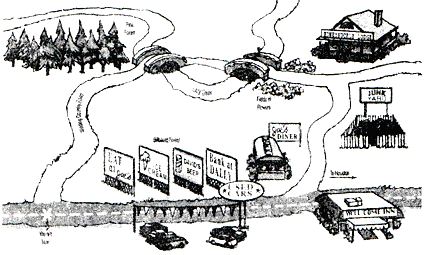
\includegraphics[height=140pt,keepaspectratio]{joe_diner.png}
\end{figure}

如果问路的请求中包括特殊要求,那么一种解决方案可能比另一种好。例如,“我要迟到了,哪条路到Joe’s Diner最快?”这时第一种方案更合适。如果要求是“有没有安静的小路可以到Joe’s Diner?”就要用第二种方案。如果没有特殊要求,那么可以根据个人喜好进行选择,不同的人面临不同的选择,最终选择的结果也不尽相同。

在评估某一问题的不同的解决方案时,一个比较标淮是效率。如果把效率当作一个非形式化的概念,会很容易认为一个程序比另一个效率更高。另一方面,也就没有机会具体考虑什么叫效率。

在实践中会发现有些程序运行得非常快,有些却很耗时。直觉告诉我们,执行得快的程序效率高,而执行慢的程序其效率相对较低。但这种直觉是有误导性的。

尽管运行时间和效率是相互关联的概念,它们并不完全相同,因为问题的内在难度是不同的。

用一个低效率的程序解决一个简单的问题所花的时间可能比用一个高效率的程序解决复杂问题所花的时间少得多。效率必须考虑到问题的难度。当谈到效率时,最好考虑到解决同一问题的不同算法的相对效率。

在计算机科学的高级课题中,衡量算法的相对效率是一个主要的课题,这个课题被称为算法分析(analysis of algorithm)。尽管理解算法分析需要用到数学知识而且要进行细致的思考,但我们还是可以通过比较几个简单算法的性能大概了解怎样进行算法分析。

\section{评估算法效率}

假设给出了解决同一问题的两个算法。要判断哪一种算法效率更高,应该怎样进行比较呢?

在某些情况下,可以利用经验进行衡量。如果想判断哪个算法能更快地解决特定问题,可以执行这两个程序,看每一个程序运行的时间。假设可以在现代计算机的计算速度下精确地测量时间,那么这种方法可以精确提供这个问题的每种解法的耗时信息。但是这种方法还是有误导的可能,尤其是当算法的运行时间取决于输入数据的时候。一个算法在输入一组数据时运行很快,也有可能在输入另一组数据时运行很慢。一些算法在有少量的输人数据时可能运行得很好,但当数据量增大时运行效果会降低很多。

在现实中,同一个问题可能有多个等价有效解决方案。在计算机科学中,关于算法的选择通常是由效率决定的。哪个算法花费的计算时间最少?哪个算法完成作业的工作量最小?这里我们指的是计算机所做的工作量。

当评估算法效率时,计算机科学家使用字母$N$表示问题规模,而不管它是怎样得出的。算法分析的核心问题是确定一个算法的运行时间是怎样随着N值变化的。当N值变大时,N和算法运行时间之间的关系被称为该算法的计算复杂性(computational~complexity)。


要比较两个算法的工作量,首先要定义一组客观的度量标准。算法分析是理论计算机科学的一个重要研究领域。下面介绍算法分析的一小部分,通过比较两个任务相同的算法,来理解算法的复杂度构成的一个从易于解决到不能解决的连续统。

程序员衡量两个不同算法执行的工作时,首先想到的是对算法编码,然后对比两个程序的运行时间。执行时间较短的算法显然是比较好的算法。但是,实际情况是,使用这种方法,只能确定程序A在特定的计算机上比程序B有效。执行时间是特定计算机特有的。当然,可以在所有可能的计算机上测试算法,但我们需要一个更通用的方法。

第二种方法是计算执行的指令输或语句数。但是,使用的程序设计语言不同,以及程序员的个人风格不同,都会对这种衡量方法有影响。为了标准化这种衡量方法,可以计算算法中执行关键的循环的次数。如果每次迭代的工作量相同,那么这种方法就给我们提供了算法效率的有效衡量标准。

另一种方法是把算法中的一个特定基础操作分离出来,计算这个操作执行的次数。例如,假设要求一个整数列表中的元素的和。要衡量所需的工作量,就要计算整数加法操作的次数。对于有100个元素的列表,需要99次加法运算。但要注意,并非真的要去计算加法运算的次数,它是列表中的元素个数($N$)的函数。因此,可以用$N$表示加法运算的次数,对于有$N$个元素的列表,需要$N-1$次加法运算。这样现在就可以比较一般情况的算法性能,而不必只是比较特定列表大小的情况了。

实际上,关于算法效率的大部分真知灼见是帮助我们理解一个算法的性能怎样随着问题规模的变化而改变。
对很多算法来说,问题规模是很容易量化的。例如,在经典算法(如测试素数或找最大公因子)中随着数字变大,运算速度会大大降低。在这类算法中,数字的大小提供了一个衡量问题规模的合适标准。对于操作数组的算法(如排序算法),可以把数组中的元素个数作为问题的规模。

\section{评估选择排序算法的效率}

选择排序算法有很多优点。首先,它的算法很容易理解;其次,它解决了排序这个问题。但是,还存在其他一些更有效的排序算法。而且,效率最高的排序算法需要很高的技巧。

通过评估算法的效率,可以进一步改进算法。尽管到目前为止我们还不能充分改善选择排序的效率,但现在正在考虑它的效率到底如何。

一个很有趣的问题就是确定用选择排序算法对某一输入数组进行排序需要多长时间,这里有两种方法可供参考:

(1)可以运行该程序看它需要多少时间。不过可以使用计算机内部的时钟得到结果。

由于程序在现代计算机中运行的速度非常快,通常运行的时间不到一秒,因此用秒表根本不可能测出运行的时间。

(2)可以更一般地考虑程序的操作,对它的行为进行量化。

\section{测试程序的运行时间}

为了确定运行一个程序需要的时间,常用的方法是用系统库来记录所需要的时间。ANSI接口time.h输出一个名为clock的过程,它能返回执行某一程序所用的以计算机处理单元为单位的时间量。clock函数返回的类型是与机器相关的时钟单位,但是可以通过以下的表达式将它转化成以秒来计算的时间形式:
\verb|(double) clock() / CLOCKS_PER_SEC|
如果把开始时间和结束时间分别存储于变量start和finish中,可以用下列代码计算执行一个操作所需的时间:
\begin{verbatim}
double start, finish, elapsed;
start = (double) clock() / CLOCKS_PER_SEC;
. . . 执行某些操作
finish = (double) clock() / CLOCKS_PER_SEC;
elapsed = finish – start;
\end{verbatim}

于是就可以用上述方法计算选择排序算法的运行时间。对大小不同的数组调用SortIntegerArray函数所需要的时间见下表。
\begin{table}[!h]
\centering
\caption{选择排序算法的运行时间(以毫秒为单位)}
\begin{tabular}{|l|l|l|l|}
\hline
N 			& 运行时间(毫秒)	& N 				& 运行时间(毫秒)			\\
\hline
10			& 0.13				& 100				& 9.67						\\
\hline
20			& 0.33				& 200				& 37.33						\\
\hline
30			& 1.00				& 400				& 146.67						\\
\hline
40			& 1.47				& 800				& 596.67						\\
\hline
50			& 2.40				& 					& 								\\
\hline
\end{tabular}
\end{table}


在这张表中,$N$表示数组中元素的个数,而“运行时间”列表示使用选择排序算法对相应的数组进行排序所需要的时间(时间单位为毫秒)。

这张表显示了一个有趣的现象。当$N$很小时,选择排序算法需要的时间很少,但随着$N$的增大,执行选择排序算法需要的时间显著增加。举个例子来说,如果数组包含30个值,SortIntegerArray排序这个数组需要1毫秒,当达到800个值时,需要的时间超过0.5秒。而商业应用通常需要对10~000、100~000甚至更多的数进行排序。对这种规模的数组,选择排序算法的速度将慢得惊人。

\section{选择排序的算法分析}

要理解实现某种算法的程序的运行时间的变化规律,首先要明白算法的工作原理。考虑选择排序的时间数据,当$N$为50时,执行算法需要2.4毫秒,而当$N$为100时,需要的执行时间为9.67毫秒,差不多是$N$为50时需要时间的4倍。

我们从表中其他部分也可以得到这样的结论:数组的元素个数增加一倍,那么所需要的时间是原来的4倍。我们把这个排序算法称为具有平方律(quadratic)的性质,即执行时间和输入数组大小的平方成正比。

选择排序算法具有平方律性质的事实其实并不奇怪,只要思考一下算法的执行过程就可以理解。在对一个具有8个元素的数组进行排序时,该算法需要执行8次外层for循环。第一个循环周期找出8个数中的最小值,下一个循环周期则在剩下的7个元素中找到最小值,依次类推。

程序执行的操作次数和该数组的个数成正比,对上面的例子,需要执行的操作的次数为:
\[8+7+6+5+4+3+2+1=36\]
更一般的情况,假如数组有N个数,选择排序需要的时间与下面的和成正比,即:
\[N+N-1+N-2+\cdots+3+2+1=\dfrac{N^2+N}{2}\]
于是,可以从上式的$N^2$中很容易看出这种平方律的性质。

各种排序算法的效率差别很大,对于具有较少元素的数组来说,使用选择排序算法这种简单的算法很合适,但对于具有较多元素的数组,该算法就不合适了。

应用数学方法预测算法效率的过程称为算法分析(analysis of algorithm),通过学习如何分析某一算法效率的问题,对于我们以后评价某一问题适合用哪种算法是非常有用的。



\chapter{大O分析}

计算机科学家用O(读作Big Oh)表示算法的计算复杂性。这个符号为大O标记,由一个大写的字母口及其后的一个用圆括号括起的公式组成,该公式表示运行时间随问题规模变化的函数。

在计算机科学中,当用操作输入的大小的函数来衡量工作量时,可以用数量级表示这个函数的近似值。字母O代表单词order(顺序),因为它用于短语on the order of,所以指的是近似值。

函数的数量级是以问题的大小为参数的函数中的最高项。因此,可以得到大O标记(Big-O Notation)的正式定义如下:
\begin{verbatim}
以函数中随着问题的大小增长得最快的项来表示计算时间(复杂度)的符号称为大O标记。
\end{verbatim}
从而使用大O分析可以根据由问题大小决定的增长速率来对比算法,从而说大O标记指出了一个程序的运行时间是怎样随着问题规模的变化而变化的,而降低一个算法的计算复杂性可以大大提高运行效率。

例如,如果
\[f(N)=N^4+100N^2+10N+50\]
那么$f(N)$的数量级是$N^4$,用大O符号表示就是$O(N^4)$。也就是说,对于较大的$N$,$N^4$在函数中占支配地位。$100N^2+10N+50$并非不重要,只是随着$N$越来越大,其他的因素就会变得无足轻重,因为$N^4$支配着这个函数的数量级。



对于大O符号(Big-O~Notation)的正式定义是,以函数中随着问题的大小增长得最快的项来表示计算时间(复杂度)的符号,从而使用大O分析可以根据由问题大小决定的增长速率来对比算法。至于为什么可以舍弃低数量级的项,可以考虑这样的例子,如果我们想要购买大象和金鱼,考虑两家宠物销售商,我们只需要对比大象的价格,金鱼的价格根本微不足道。

\begin{figure}[htbp]
\centering
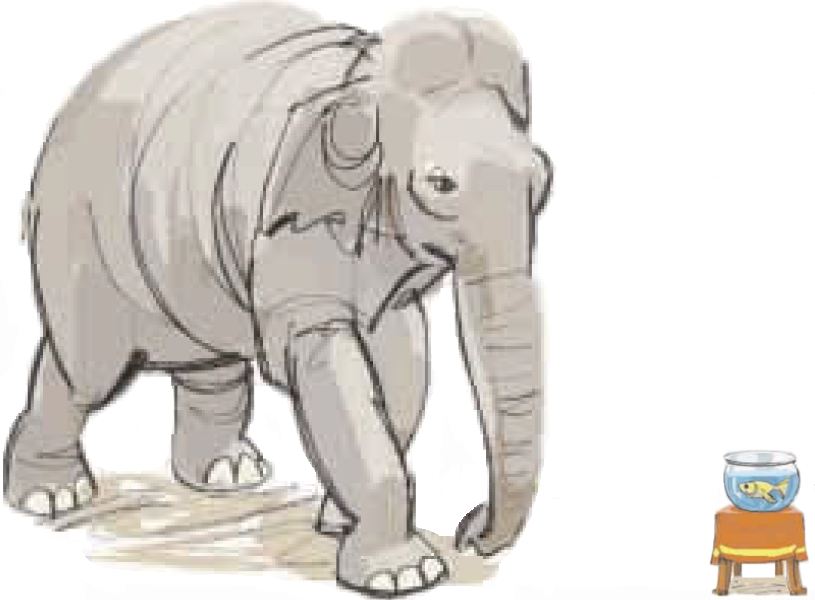
\includegraphics{elephant_goldfish.png}
\end{figure}

同样地,在算法分析中,随着问题大小增长得最快的项支配着整个函数,把其他项明显地降到了“噪音”的水平。大象太大以至于我们可以忽略金鱼。同样地,对于较大的$N$,$N^4$比$50$、$10N$,甚至$100N^2$都大得多,以至于可以忽略这些项。这并不意味着这些项对计算时间没有影响,只是说它们在$N$比较“大”时对我们的估计没有显著影响。


\section{什么是N}


$N$表示问题的大小。大多数问题都涉及到数据结构,每种结构由元素构成。我们要开发算法,把元素添加到结构中,以及修改元素,或把元素从结构中删除。用$N$可以描述这些操作的工作量,$N$是结构中的元素个数。

假设要把一个列表中的所有元素写入一个文件。这个算法的工作量是由列表中的元素个数决定的。算法如下:
\begin{verbatim}
Open the file
While more elements in list
    Write the next element
\end{verbatim}
如果$N$是列表中的元素个数,那么要实现这个任务需要的时间是($N\times $写入一个元素的时间)$+$打开文件的时间。

这个算法的时间复杂度是$O(N)$,因为执行任务所需的时间与元素个数$N$成比例(外加一点打开文件的时间)。在决定大$O$的近似值时,因为打开文件必需的时间基本是一个常量,那么算法的这个部分就相当于金鱼。如果列表中只有几个元素,打开文件的时间可能会看起来很重要,但对于较大的$N$,写入元素的操作与打开文件比起来就像大象。

算法的数量级并没有表明解决方案在计算机上运行需要花费多少微秒。有时,我们需要这种信息。例如,一个字处理程序的要求写到,该程序必须能在(特定计算机上)120秒以内对50页文档进行拼写检查。对于这种信息,就不能使用大$O$分析,而需要其他的衡量方法。

我们可以对一种数据结构的不同实现进行编码,然后运行测试,记录运行前和运行后的计算机时钟上的时间。这种基准测试可以说明,这些操作在特定的计算机上用特定的编译器执行需要花费多少时间。但大$O$分析无需引用这些因素就可以比较算法。

\section{一个比喻:家庭洗衣量}

每周一个家庭要花多少时间洗衣服?可以用下面的函数来回答:
\[f(N)=c*N\]
$N$表示家庭成员数,$c$是每个人的衣服需要花费的时间。这个函数的复杂度是$O(N)$,因为整体的洗衣时间是由家庭成员数决定的。对于不同的家庭,常量$c$可能稍有不同,这是由洗衣机的容量和他们折叠衣服的速度决定的。也就是说,两个家庭的洗衣时间可以用下面的两个函数表示:
\[f(N)=100*N\]
\[g(N)=90*N \]

现在,如果爷爷和奶奶来第一个家庭住一到两个星期会出现什么情况?洗衣时间的函数将变为:
\[f(N)=100*(N+2)\]

我们仍然说这个函数的复杂度是$O(N)$。虽然多出了两个人,漂洗、烘干和叠衣服的时间也增加了。虽然此时$N$很小(这个家庭只有妈妈、爸爸和孩子),那么增加两个人需要多花的洗衣时间还是很明显的。不过随着$N$的增加(这个家庭有妈妈、爸爸和12个孩子和一个保姆),多两个人区别就不大了。(这家的洗衣时间就像大象;而客人的洗衣时间就像金鱼。)当用大$O$比较算法时,我们关心的是$N$比较大的情况。

如果我们的问题是“我们能及时洗完衣服,赶上7:05的火车吗?”那么我们想要的是精确的答案。大$O$不能给我们这些信息,它给的是个近似值。

因此,如果$100*N$、$90*N$和$100*(N+2)$的复杂度都是$O(N)$,那么我们如何分辨哪个更好呢?用大$O$符号,我们不能回答哪个更好,对于较大的$N$,它们基本上是等价的。我们能找到更好的洗衣算法吗?如果这个家庭中了彩票,那么他们就可以在距离他们家15分钟车程(往返约为30分钟)的专业洗衣店洗衣。现在,这个函数是:
\[f(N)=30\]
这个函数的复杂度是$O(1)$,这个答案独立于家庭成员数。如果车程变为5分钟,那么该函数就变为:
\[f(N)=10\]
这个函数的复杂度仍然是$O(1)$。采用大$O$进行比较,这两种专业洗衣店的解决方案是等价的,无论有多少位家庭成员,也无论有多少客人,这个家庭用来洗衣的时间都是个常量。(这时,我们不关系专业洗衣店的时间。)


\section{常见的数量级}

考察队列软件包的原始实现,Enqueue操作的运行时间不随问题规模的变化而变化,此处问题规模可以定义为队列中当前的项数。在计算机科学中,如果一个操作所需要的时间与问题规模无关,则说该操作以恒定时间(constant~time)运行。

在大$O$标记中,恒定时间用$O(1)$表示,$O(1)$的意思是当$N$变大时,这个程序的运行时间随1的改变而改变,因为1是常数,所以当N值增加时,它并不发生变化,这也是恒定时间操作的一个显著特征。

$O(1)$又叫做有界时间,即工作量是个常数,不受问题大小的影响。给具有$N$个元素的数组中的第$i$个元素赋值,复杂度是$O(1)$,因为可以通过索引直接访问数组中的元素。虽然有界时间通常又叫做固定时间,但工作量却不必一定是固定的,它只是有一个常量界限而已。

在下面的Dequeue操作中行为有所不同,Dequeue的实现用下列for循环把该队列中每一项向数组头方向移一步:
\begin{verbatim}
for(i = 1; i < queue -> len; i ++){
     queue -> array[i - 1] = queue -> [i];
}
\end{verbatim}
如果队列包含$N$项,这个for循环就要执行$N$个周期。随着$N$的增加,for循环执行时间成正比例增加。

如果N很大,for循环的消耗远远超过循环外所有操作的消耗,因为无论$N$值多大,这些循环外的操作往往只执行一次。这样一来,在某一范围内随着$N$变大,Dequeue操作的运行总时间会随N的增加而增加。如果一个操作的运行时间与问题规模成正比,则称此操作以线性时间(linear~time)运行,用大$O$标记表示为$O(N)$,即工作量是一个常数乘以问题的大小,输出具有$N$个元素的列表中的所有元素,复杂度是$O(N)$。在无序列表中检索一个值的复杂度也是$O(N)$,因为必须检索列表中的每一个值。

前面提到的队列软件包的环缓冲区实现的优点在于,它把Dequeue操作的运行时间由线性时间降低为恒定时间,即从$O(N)$到$O(1)$。如果$N$值很大,这种优势是很明显的。另一方面,使一个线性算法以恒定时间运行所节省的时间远远小于在更复杂的算法中进行改进带来的省时效果。

$O(N)$叫做线性时间,即工作量是一个常数乘以问题的大小。输出具有$N$个元素的列表中的所有元素,复杂度是$O(N)$。在无序列表中检索一个值的复杂度也是$O(N)$,因为必须检索列表中的每一个元素。

\section{再看选择排序算法}

在选择排序算法的实现中,如果给出一个有$N$个元素的数组,选择排序算法要访问每一个数组元素的位置,并确定该位置应该存放的值。为了找到合适的值,算法必须查找剩下的数组元素并找到最小的值。这样,算法用$N$步填好第一个位置,用$N-1$步填人第二个位置,依次类推,因此,总的运行时间与
\[N + N-1 + N-2 + ... + 3 + 2 + 1\]
成正比,该公式也是:$\dfrac{N^2+N}{2}$

当使用大O标记来估计一个算法的计算复杂性时,目的是提供一种简化手段,以便衡量当N变大时,N的变化是如何影响算法的性能。因为大O标记并非一种精确的量化手段,所以我们最好能简化括号中的表达式,以便用最简单的形式量化算法的行为。

对圆括号里的公式应用下列步骤,可以简化大O标记。

(1)消去公式中任何随N变大而变得无足轻重的项。

例如,在选择排序算法中,当N值增加时,N2很快比N大很多。选择排序的运行时间因此更依赖于N2项。因此,当使用大O标记时,可以忽略N而重点关注N2。

(2)消去任何常数系数。

当计算计算复杂性时,最关心的是对于不同的N值,各种算法的相对运行时间。如果使用一个比率表示相对时间,那么分子和分母中的常数系数都会被消去。常数系数对于相对运行时间是没有影响的,所以可以在用大O标记时删去常数系数。

因此,用下列公式描述选择排序算法的计算复杂性是不合适的。
\[O\bigg(\dfrac{N^2+N}{2} \bigg)\]
因为上面这个表达式包含了N这个项,它对于N2来说是可忽略的。也不能写成下面这样:
\[O\bigg(\dfrac{N^2}{2} \bigg)\]
因为应该消去常数项。因此,最终用来表示选择排序的复杂性的表达式应为:
\[O(N^2)\]
$O(N^2)$叫做二次时间,这类算法通常要应用N次线性算法。大多数简单排序算法的时间复杂度都是$O(N^2)$。

运行性能为$O(N^2)$表示的算法被称为以平方时间(quadratic~time)运行。平方复杂度的基本特征是,如果问题规模翻倍,则运行时间会增加4倍。选择排序是一个平方算法,随着要排序的数组变大,这个性能会严重地限制它的实用性。

大多数简单排序算法的时间复杂度都是$O(N^2)$,即这类算法通常要应用$N$次线性算法。

\section{分而治之策略}

从另一种角度思考,选择排序算法的平方复杂度也提供了某种方便。已知把一个平方问题的规模加倍,运行时间会增加4倍。这种特性使得选择排序无法适用于较大的数组。

然而,反过来,如果把一个平方问题的规模除以2,它的运行时间同样将减少到原来的四分之一。因此,如果把一个大数组分成两半,再用选择排序算法分别对每一半数组元素排序,结果对两个子数组排序所用时间是对整个数组排序所用时间的一半。(每一个子数组花费原时间的四分之一,则排序两个这样的子数组花费两个四分之一的时间。)

分别排序一个数组的两半简化了排序整个数组的问题,从而大幅度减少了总耗时。更重要的是,一旦发现怎样在一个层面上改善性能,就能用同样的算法递归地为每一个子数组排序。

把一个问题分解成基本相等的子问题,并递归地解决每一个子问题,这样的递归算法称为分而治之(divide-and-conquer)算法。

要确定分而治之方法是否适用于排序问题,关键问题在于将一个数组分成两个子数组并对两个子数组分别排序是否有助于解决原问题。为使这个问题更具体,下面讨论一个有8个元素的数组的例子:
\begin{figure}[!h]
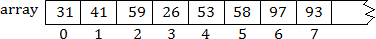
\includegraphics{array_8.png}
\end{figure}

如果把这个有8个元素的数组分成2个有4个元素的数组,然后对每一个子数组排序。记住,应用递归信任可以假定递归调用能正确运行,这样将得到如下结果:
\begin{figure}[!h]
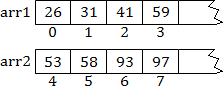
\includegraphics{array_1_2.png}
\end{figure}
这样做的目的是把这些值从子数组中取出来,并以正确顺序放回原数组:
\begin{figure}[!h]
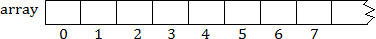
\includegraphics{array_8_1.png}
\end{figure}

\section{合并两个数组}

把已排序的子数组重组成一个完整数组比排序本身要简单,这种技术叫合并(merging)。它基于一个事实,即完整的排序的第一个元素只能是arr1或arr2的第一个元素,但要取更小的那个元素作为第一个元素。

在这个例子中,新数组中的第一个元素是arr1中的26。如果把这个元素放入array[0],实际上,就是把它从arr1中划掉,结果得到以下结构:
\begin{figure}[!h]
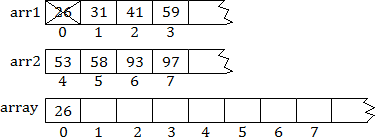
\includegraphics{arr1_arr2.png}
\end{figure}
接着,下一个元素只能是两个子数组中第一个未用过的元素。把arr1中的31和arr2中的53比较,并选择前者:
\begin{figure}[!h]
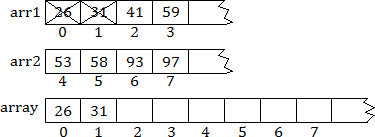
\includegraphics{arr1_arr2_1.png}
\end{figure}
可以继续在arr1、arr2中选择较小值的过程,直到整个数组被填满为止。

\section{合并排序算法}

合并操作与递归分解相结合,产生了一个新的排序算法——合并排序(merge sort),实现这个算法的方法很简单。函数SortIntegerArray首先判定数组的大小。如果数组没有元素或只有一个元素,那么数组必然已经被排过序。因此这个条件定义了这种简单情况。然而,如果数组包含的元素多于1个,就需要执行下列步骤:

(1)把数组分成两个较小的子数组,每一个数组的大小是原数组的一半。

(2)递归调用SortIntegerArray为每一个小数组排序。

(3)合并两个小数组,写回原数组。

函数SortIntegerArray本身的代码如下:
\begin{verbatim}
void SortIntegerArray(int array[], int n)
{
    int i, n1, n2;
    int *arr1, *arr2;
    if(n > 1){
        n1 = n / 2;
        n2 = n – n1;
        arr1 = NewArray(n1, int);
        arr2 = NewArray(n2, int);
        for(i = 0; i < n1; i ++) arr1[i] = array[i];
        for(i = 0; i <n2; i ++) arr2[i] = array[n1 + i];
        SortIntegerArray(arr1, n1);
        SortIntegerArray(arr2, n2);
        Merge(array, arr1, n1, arr2, n2);
        FreeBlock(arr1);
        FreeBlock(arr2);
    }
}
\end{verbatim}
在这个实现中,arr1和arr2是较小的数组,它们有效长度分别为n1和n2,所有困难的工作都由Merge完成,Merge实现如下:
\begin{verbatim}
static void Merge(int array[], int arr1[], int n1, int arr2[], int n2)
{
    int p, p1, p2;
    p = p1 = p2 = 0;
    while(p1 < n1 && p2 < n2){
        if(arr1[p1] < arr2[p2]){
            array[p ++] = arr1[p1 ++];
        }else{
            array[p ++] = arr2[p2 ++];
        }
    }
    while(p1 < n1) array[p ++] = arr1[p1 ++];
        while(p2 < n2) array[p ++] = arr2[p2 ++];
}
\end{verbatim}
Merge函数的参数有目标数组以及较小的数组arr1和arr2,还有它们的有效长度n1和n2。

下标p1和p2标志着每一个子数组的进度,p是array的下标。在每一个循环周期中,函数从arr1或arr2中选择一个较小元素,把该值复制到array中。一旦任何一个子数组的元素用完,该函数就直接把另一个子数组中剩下的元素复制到目标数组中,不用再进行比较测试了。实际上,因为知道当第一个while循环结束时,有一个子数组已经为“空”,所以函数把另一个数组剩下的部分复制到目标位置即可。一个子数组为空后,则相应的while循环将不用执行。

\section{合并排序的计算复杂性}

下面讨论通过函数SortIntegerArray实现分而治之的策略时的效率,虽然可以通过为数组排序并计时来测量其效率,但是从考虑计算复杂性着手会更有帮助。

当调用合并排序的实现(SortIntegerArray函数)为N个数字排序时,运行时间可分成下面两部分:

(1)在当前的递归分解层次上,执行操作所需的所有时间。

(2)执行递归调用的时间。

在递归分解的最上面一层,执行非递归操作所消耗的时间与N成正比。SortIntegerArray的两个for循环一起形成N个循环周期,对Merge的调用填满了原数组的N个位置。如果把这些操作加起来,去掉常量因子,会发现任何一次SortIntegerArray调用的复杂性(如果不考虑其中的递归调用)需要O(N)次操作。

但是递归操作的代价又如何呢?要排序一个大小为N的数组,必须递归地排序两个大小为N / 2的数组。为每一个子数组排序都需要同样的时间。如果应用同样的逻辑,则很快就能够确定每一个递归调用需要的时间正比于该层上的N / 2,加上递归调用所需时间。继续同样的过程,直到到达一种简单情况,即子数组只有一个元素或无元素为止。

解决这个问题所需的总时间是递归分解的每一层所消耗的时间之和。总的来说,分解的结构如下图所示。
\begin{figure}[!h]
\centering
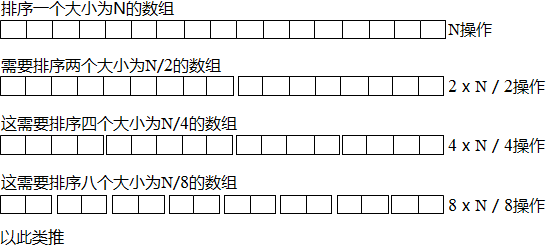
\includegraphics[height=120pt,keepaspectratio]{sort_merge.png}
\caption{合并排序的递归分解}
\end{figure}
当沿着递归层次向下执行时,数组越来越小,但数组个数却越来越多。然而,每一层的工作量总是和N直接成正比的。因此,确定工作总量就转化为确定层数的问题。

在递归层次结构的每一层中,$N$值都除以2。总层数等于你在$N=1$之前将州除以2的次数。

用数学术语表述这个问题,就是说必须找到一个这样的k值,使得
\[N=2^k\]
解这个方程,得到k的值为:
\[k=\log_2^N\]
因为层数为$\log_2^N$,且每一层的工作量与N成正比,所以总工作量与$Nlog_2^N$成正比。

在其他学科中,对数的底数通常为10(常用对数)或数学常量e(自然对数),但在计算机科学中,总是使用二进制对数(binary~logarithm),即以2为底数的对数。由于对数计算底数不同,而底数又是常数,因此,当谈到计算复杂性的问题时,可以像以前那样忽略对数的底数。这样合并排序的计算复杂性可以写为:
\[O(N\log N)\]

\section{比较平方复杂性与NlogN复杂性的性能}

至于$O(N\log N)$的性能到底有多好,可以把它和$O(N^2)$作比较。对于不同的$N$值,这两个函数的值如下表所示。
\begin{table}[!h]
\centering
\caption{ $N^2$和$N\log N$的比较}
\begin{tabular}{|l|l|l|}
\hline
$N$				& $N^2$			&  $N\log N$		\\
\hline
10					& 100				& 33				\\
\hline
100 				& 10~000		& 664				\\
\hline
1~000				& 1~000~000	& 9~965			\\
\hline
10~000			& 100~000~000& 132~877		\\
\hline
\end{tabular}
\end{table}

在这个表中,随$N$值变大,两个列中的数值也增大,但$N^2$一栏增大的速度比$N\log N$栏增大得快,因此基于$N\log N$算法的排序策略能够更广泛地应用于各种大小的数组。

为了在实践中证实上表中的理论结果,因为大$O$标记消去了所有的常量,所以选择排序可能对于有某种规模的问题来说更有效。对不同大小的数组分别运行选择排序和合并排序,并测量实际运行时间,得到下表中的结果。因为计算机的速度有所不同,这些数值可能随机器的不同而有所变化,但基本的模式应该是一样的。
\begin{table}[!h]
\centering
\caption{排序算法的运行时间(以秒为单位)}
\begin{tabular}{|l|l|l|}
\hline
$N$			& 选择排序				& 合并排序			\\
\hline
10 				& 0.000~13				& 0.000~94			\\
\hline
100 			& 0.009~67				& 0.012				\\
\hline
1~000 		& 1.08					& 0.14				\\
\hline
10~000		& 110.0					& 1.6					\\
\hline
\end{tabular}
\end{table}

对于有10个元素的数组来说,选择排序比合并排序快4倍。对于有100个元素的数组来说,选择排序还是较快,但只快一点点。但当达到10~000个元素时,选择排序比合并排序慢70倍,需要将近2分钟来完成。

这些增长系数正是我们想从计算复杂性中得到的。在将数组大小乘以10时,选择排序所需时间应增加100倍,而表中数据验证了这一点。对于合并排序,将数组大小增大10倍,将使运行时间增加为原来的10倍多一点,在表中的数据同样可以观察到这个结果。

总结:

$O(1)$叫做有界时间,即工作量是个常数,不受问题大小的影响。给具有$N$个元素的数组中的第$i$个元素赋值,复杂度是$O(1)$,因为可以通过索引直接访问数组中的元素。虽然有界时间通常又叫做固定时间,但工作量却不必一定是固定的,它只是有一个常量界限而已。

$O(\log_2^N)$叫做对数时间,即工作量是问题大小的对数。每次都把问题的数据量减少一半的算法通常都属于这个类别。用二分检索法在有序列表中查找一个值,复杂度就是$O(\log_2^N)$。

$O(N)$叫做线性时间,即工作量是一个常数乘以问题的大小。输出具有$N$个元素的列表中的所有元素,复杂度是$O(N)$。在无序列表中检索一个值的复杂度也是$O(N)$,因为必须检索列表中的每一个元素。

$O(N\log_2^N)$叫做$N\log_2^N$时间,这类算法通常要应用$N$次对数算法。比较好的排序算法(如快速排序、堆排序和合并排序)的复杂度都是$N\log_2^N$。也就是说,这些算法能用$O(N\log_2^N)$的时间把一个无序列表转换成有序列表,不过快速排序算法对于某些输入数据的时间复杂度是$O(N^2)$。

$O(N^2)$叫做二次时间,这类算法通常要应用$N$次线性算法。大多数简单排序算法的时间复杂度都是$O(N^2)$。

$O(2^N)$叫做指数时间,这类算法非常耗时。在下表中可以看到,随着$N$的增长,指数时间增长得非常快。在棋盘中的每一格放稻谷的例子就是指数时间算法,在这个例子中,问题的大小就是稻谷的颗粒数。(还要注意的是,最后一列的值增长得非常快,以至于这个数量级的问题所需的计算时间超出了预计的宇宙生命期限。)

\begin{table}[!h]
\centering
\caption{增长率的对比}
\begin{tabular}{|p{25pt}|p{25pt}|p{25pt}|p{25pt}|p{40pt}|p{160pt}|}
\hline
$N$	&	$\log_2^N$	& $Nlog_2^N$	& $N^2$	& $N^3$	& $2^N$	\\
\hline
1		& 	0				& 1				& 1		& 1		& 2		\\
\hline
2		& 1				& 2				& 4		& 8		& 4		\\
\hline
4		& 2				& 8				& 16		& 64		& 16		\\
\hline
8		& 3				& 24				& 64		& 512		& 256		\\
\hline
16		& 4				& 64				& 256		& 4096	& 65536	\\
\hline
2		& 5				& 160				& 1024	& 32768	& 4294967296\\
\hline
64		& 6				& 384				& 4096	& 262144& 在超级计算机上约为5年\\
\hline
128	& 7				& 896				& 16384	& 2097152& 以纳秒计约为宇宙年龄的600000倍(估计为60亿年)\\
\hline
256	& 8				& 2048			& 65536	& 16777216	& $-$			\\
\hline
\end{tabular}
\end{table}

$O(n!)$叫做阶乘时间。这类算法甚至比指数时间的算法更耗时。货郎担这个图论问题就是一个阶乘时间算法。

\section{多项式时间算法}

数量级是问题大小的多项式的算法叫做多项式时间算法(polynomial-time~algorithms)。多项式是两个或多个代数项的和,每个代数项是一个常量乘以一个或多个变量的非负整数次幂。因此,多项式算法就是数量级(或复杂度)能够用问题大小的幂表示的算法。算法的大$O$符号是多项式中的最高次幂。所有的多项式时间算法都被定义为$P$类(class~P)算法。

把常见的复杂度量级看作一个箱子,我们可以以此对算法复杂度排序。如下图所示:

\begin{figure}[!h]
\centering
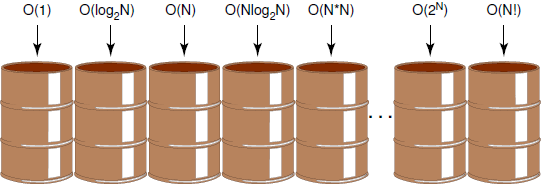
\includegraphics[height=100pt,keepaspectratio]{class_p_box.png}
\caption{复杂度的顺序}
\end{figure}

对于较小的问题,一个箱子中的算法可能真的比下一个更有效的箱子中的等价算法快。随着问题增大,不同箱子中的算法之间的差别会随之增加。在选择同一个箱子中的算法时,就不能再忽略金鱼了。


\section{算法分类}

可以引入箱子的形状来表示常见的算法的数量级,而事实上最右边还应该有一个箱子,存放的是不能解决的算法。

下面将重组这些箱子,把所有多项式算法放在$P$类箱子中,把指数和阶乘算法放在一个箱子中,再加一个不能解决的算法的箱子,如下图所示:

\begin{figure}[htbp]
\centering
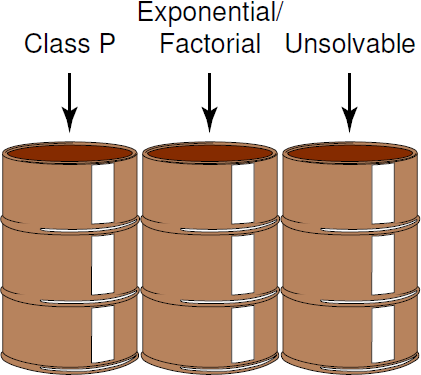
\includegraphics{p_class_box_1.png}
\caption{重组的算法分类}
\end{figure}

在重组后的算法分类中,虽然中间箱子中的算法是有解决方案的,但由于无论数据量大小,它们都要执行很长的时间,所以它们被称为{\heiti 难处理的算法。}

并行计算机体系结构出现以后,如果同时使用足够多的处理器,某些问题就有可能在合理的时间(多项式时间)得到解决了。因此,如果使用足够多个处理器,就能在多项式时间内解决的问题叫做$NP$类问题(Class~NP~problems)。相应地,用一个处理器能在多项式时间内解决的问题叫做$P$类问题(Class~P~problems)。

显然,$P$类问题也是$NP$类问题。理论计算学中的一个未决问题是,只有用多个处理器才能解决的$NP$类问题是否也是$P$类问题。也就是说,这些问题是否存在多项式算法,而目前我们还未发现(发明)。我们不知道这个答案,计算机科学的理论研究这一直在寻求这些的解决方案。

仅仅是判断$P$类是否等价于$NP$类的问题已经被简化为找到其中一个算法的解决方案。有一类的特殊的问题叫做$NP$完全问题(NP-complete~problems)。这些问题属于$NP$类,它们的属性可以互相映射。如果找到了这个类中的一个算法的单处理器多项式时间解决方案,那么其他所有算法都会存在这样的解决方案,因为一个解决方案可以映射到其他所有问题的解决方案。

在我们对复杂度的陈述中加入了新的$NP$类复杂度箱子后,这个箱子和P类箱子相邻的一边用虚线标示了出来,因为它们实际上是一个箱子,算法分类变成如下图所示:

\begin{figure}[htbp]
\centering
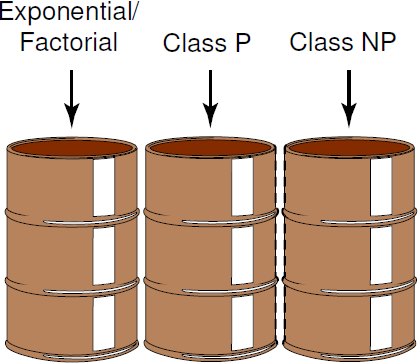
\includegraphics{np_class_box.png}
\caption{加入了NP类}
\end{figure}



\section{货郎担问题}

一个经典的$NP$类问题叫做货郎担问题。一个货郎要走访他的销售区域内的所有城市。为了有效地走访每个城市,他想找到一条路线,在返回起点之前,要经过且只经过每个城市一次。可以用图的顶点表示城市,图的边表示城市间的路。每条边上标有城市之间的距离。这个解决方案成了著名的图论算法,它的单处理器解决方案的复杂度是$O(n!)$。

\chapter{图灵机}

Alan~Turing在20世纪30年代开发了计算机器的概念,他的兴趣并非实现这台机器,而是用它作为一种模型来研究计算的限度。图灵机就是一种抽象数学模型,本质上它与硬件毫无关系。图灵机为计算理论的主要领域奠定了基础,现在分析图灵机的功能是所有学习计算机科学的学生的理论学习的一部分。

Turing所做的就是构想一台假想机,这是一台类似于打字机的简单装置,能够扫描或读取一条理论上无限长的带子上的指令。这台扫描器从带子上的一个方格移到下一个方格,响应序列的指令,并修改它的机械响应,Turing证明了这种过程的输出可以复制人类的逻辑思维。

\begin{figure}[htbp]
\centering
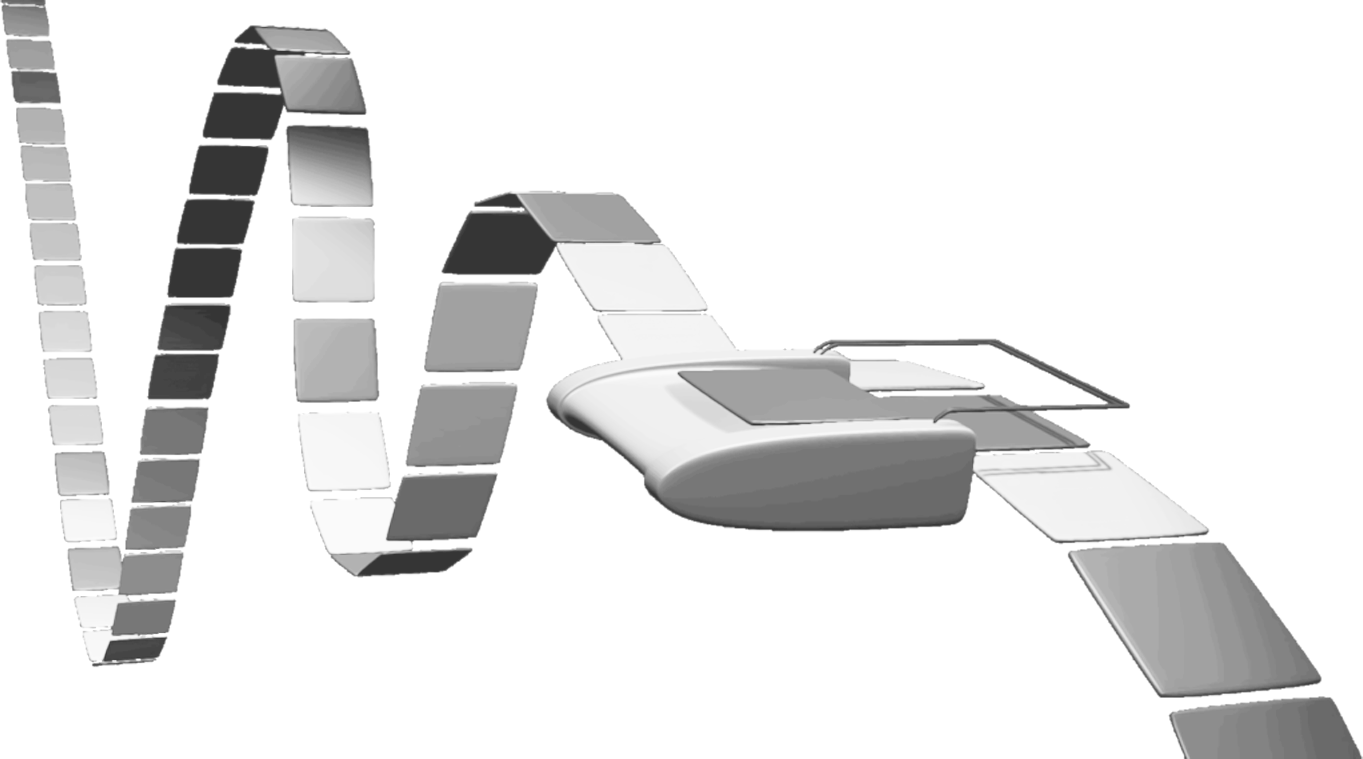
\includegraphics[height=100pt,keepaspectratio]{alan_turing.png}
\end{figure}

这种假想的装置的名字就是——图灵机,Turing的另一个构想也是如此。由于机器的行为是由带子上的指令控制的,改变这些指令,就可以使这台机器执行各种功能。换句话说,采用不同的带子,同一台机器既可以执行运算,又可以下棋,还可以执行其他所有具有计算性的任务,因此这个装置得到了一个新的名字——通用图灵机。

现代计算机的诞生汇集了无数的构想和高级技术,很难把它的发明归功于某个人。不过,每个在使用计算机的人,都在使用具体化了的图灵机。

图灵机由具有读写头的控制部件构成,能够在无限的带子上读写符号,带子被分成了单元。图灵机的基础是一个人用铅笔和橡皮在长长的纸带上进行简单的运算,纸上的每一行(一个单元)包含一个有限字符集中的符号。从第一行开始,这个人分析其中的符号,或者保留它,或者用字符集中的另一个字符替换它。然后他移到下一行,重复上述操作。

图灵机的控制部件模拟了这个人。人的决策过程由控制部件能执行的一系列指令表示。每个指令可以:
\begin{compactitem}
\item 从带子上的一个单元读取一个符号;
\item 把一个符号写入带子上的一个单元;
\item 使带子向左移动一个单元,或向右移动一个单元,或者保持不动。
\end{compactitem}

如果我们允许一个自己替换符号,这些动作其实是模拟了一个使用铅笔的人。

为什么这样一个简单的机器(模型)这么重要呢?一个广为接受的说法是任何能直观计算的问题都能被图灵机计算。这个说法叫做Church-Turing理论,以Turing和Alonzo Church的名字命名,后者开发了另一个类似的模型——$\lambda$演算。

从Church-Turing理论我们可以得出这样的结论,如果证明了一个问题的图灵机解决方案不存在,那么这个问题就是不可解决的。


\chapter{停机问题}

计算(程序)终止并不总是很明显的。比如不同的循环类型中,有些循环会明显地终止,而有的则不会(无限循环),还有些循环是根据输入的数据或循环中发生的计算终止的。在一个程序运行的过程中,很难分辨它是进入了无限循环还是需要更多时间来运行。

因此,如果可以预言一个具有特定输入的程序不会落入无限循环,是非常有用的。停机问题(halting~problem)以下面的方式重新阐述了这个问题,即\verb|给定一个程序和它的输入,确定该程序采用这样的输入最终是否能停止|。

最明显的方法是用特定的输入运行程序,看会发生什么情况。如果它停止了,答案是显而易见。如果它不停止呢?一个程序要运行多久才能判定它落入了无限循环?显然,这种方法有问题。遗憾的是,其他的方法也都有问题。这个问题是不可解决的。这个断言的证明是“没有图灵机程序可以确定一个程序是否在指定的输入下会停止。”

那么如何证明一个问题是不可解决的,或者只是我们还没找到解决方案而已呢?可以尝试每种提出的解决方案,证明每种方法都有问题。由于已知的解决方案可能很多,而且还有很多是未知的,所以这种方法看来行不通。然而这种方法构成了图灵解决方案的基础。在这个证明中,就是从提出的解决方案入手,然后证明它们是行不通的。

假设存在一个图灵程序SolvesHaltingProblem,对于任何程序Example和输入SampleData,它都能确定Example采用SampleData是否会停止。也就是说,程序SolvesHaltingProblem以程序Example和输入SampleData作为参数,如果Example能停止,则输出“Halts”,如果Example具有无限循环,就输出“Loops”。下图展示了这种情况:

\begin{figure}[!h]
\centering
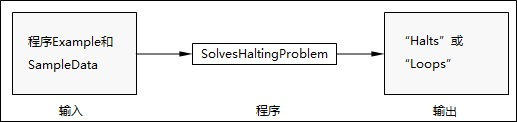
\includegraphics[scale=1.75]{halting_problem_program.png}
\caption{为解决停机问题提出的程序}
\end{figure}

在计算机中,程序(指令)和数据是相似的,都是位组合。程序和数据的区别在于控制部件如何解释位组合。因此,如果把Example自身作为SampleData,那么SolvesHaltingProblem就要以Example程序和它的副本作为参数,来判断Example以其自身作为输入是否会停止。如下图所示:

\begin{figure}[!h]
\centering
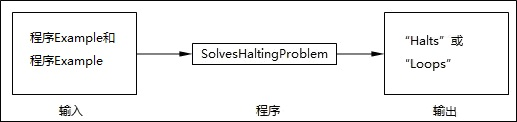
\includegraphics[scale=1.75]{halting_problem_program1.png}
\caption{为解决停机问题提出的程序}
\end{figure}

现在我们构造一个新程序NewProgram,以Example作为程序和输入数据,采用SolvesHaltingProblem的算法,如果Example会停止,就输出“Halts”,如果Example具有无限循环,就输出“Loops”。如果输出了“Halts”,NewProgram将创建一个无限循环;如果输出的是“Loops”,NewProgram将输出“Halts”。下图展示了这种情况:

\begin{figure}[!h]
\centering
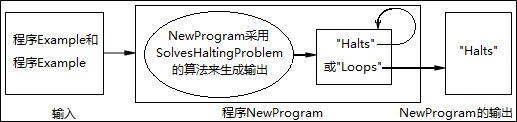
\includegraphics[scale=1.75]{new_halting_problem_program.png}
\caption{NewProgram的构造}
\end{figure}

这个证明就是,把SolvesHaltingProblem应用到NewProgram上,以NewProgram作为输入数据。如果SolvesHaltingProblem输出“Halts”,那么NewProgram就落入了无限循环。如果SolvesHaltingProblem输出“Loops”,NewProgram将输出“Halts”并停止。无论哪种情况,SolvesHaltingProblem所给答案都是错的。由于SolvesHaltingProblem至少会对一种情况给出错误答案,所以它不适用于所有情况。因此,任何提出的解决方案都是有问题的。

\clearpage
\bibliography{csnotes}
\bibliographystyle{plainnat}






















